% v2-acmsmall-sample.tex, dated March 6 2012
% This is a sample file for ACM small trim journals
%
% Compilation using 'acmsmall.cls' - version 1.3 (March 2012), Aptara Inc.
% (c) 2010 Association for Computing Machinery (ACM)
%
% Questions/Suggestions/Feedback should be addressed to => "acmtexsupport@aptaracorp.com".
% Users can also go through the FAQs available on the journal's submission webpage.
%
% Steps to compile: latex, bibtex, latex latex
%
% For tracking purposes => this is v1.3 - March 2012

\documentclass[prodmode,acmtecs]{acmsmall} % Aptara syntax

% Package to generate and customize Algorithm as per ACM style
\usepackage[ruled]{algorithm2e}
\renewcommand{\algorithmcfname}{ALGORITHM}
\SetAlFnt{\small}
\SetAlCapFnt{\small}
\SetAlCapNameFnt{\small}
\SetAlCapHSkip{0pt}
\IncMargin{-\parindent}

\usepackage[english]{babel}
\usepackage{tikz}
\usetikzlibrary{positioning}
\usepackage[pass]{geometry}
\usepackage{graphicx}
\usepackage{epsfig}
\usepackage{url}
\usepackage{color}
\definecolor{nodecolor}{RGB}{202,202,202}
\newlength\framesep
\setlength\framesep{16pt}
\pgfdeclarelayer{background}
\pgfsetlayers{background,main}
\pgfkeys{
	/tikz/node distance/.append code={
		\pgfkeyssetvalue{/tikz/node distance value}{#1}
	}
}

\widowpenalty=10000
\clubpenalty=10000

% Metadata Information
\acmVolume{9}
\acmNumber{4}
\acmArticle{39}
\acmYear{2010}
\acmMonth{3}

% Copyright
%\setcopyright{acmcopyright}
%\setcopyright{acmlicensed}
%\setcopyright{rightsretained}
%\setcopyright{usgov}
%\setcopyright{usgovmixed}
%\setcopyright{cagov}
%\setcopyright{cagovmixed}

% DOI
\doi{0000001.0000001}

%ISSN
\issn{1234-56789}

% Document starts
\begin{document}

% Page heads
\markboth{G. Zhou et al.}{A Multifrequency MAC Specially Designed for WSN Applications}

% Title portion
\title{Total Platform Cyber Protection}

%TODO Adam: Not sure if anon submission so just leaving like this for now
\author{
%First Author
%\affil{Arizona State University}
%Second Author
%\affil{Arizona State University}
%Third Author
%\affil{Arizona State University}
%Fourth Author
%\affil{Arizona State University}
%Fifth Author
%\affil{Arizona State University}
%Sixth Author
%\affil{Arizona State University}
%Seventh Author
%\affil{Arizona State University}
}
% NOTE! Affiliations placed here should be for the institution where the
%       BULK of the research was done. If the author has gone to a new
%       institution, before publication, the (above) affiliation should NOT be changed.
%       The authors 'current' address may be given in the "Author's addresses:" block (below).
%       So for example, Mr. Abdelzaher, the bulk of the research was done at UIUC, and he is
%       currently affiliated with NASA.

% TODO Sai: Discuss story with yeganeh and get a nice little abstract here
\begin{abstract}
Multifrequency media access control has been well understood in
general wireless ad hoc networks, while in wireless sensor networks,
researchers still focus on single frequency solutions. In wireless
sensor networks, each device is typically equipped with a single
radio transceiver and applications adopt much smaller packet sizes
compared to those in general wireless ad hoc networks. Hence, the
multifrequency MAC protocols proposed for general wireless ad hoc
networks are not suitable for wireless sensor network applications,
which we further demonstrate through our simulation experiments. In
this article, we propose MMSN, which takes advantage of
multifrequency availability while, at the same time, takes into
consideration the restrictions of wireless sensor networks. Through
extensive experiments, MMSN exhibits the prominent ability to utilize
parallel transmissions among neighboring nodes. When multiple physical
frequencies are available, it also achieves increased energy
efficiency, demonstrating the ability to work against radio
interference and the tolerance to a wide range of measured time
synchronization errors.
\end{abstract}


%
% The code below should be generated by the tool at
% http://dl.acm.org/ccs.cfm
% Please copy and paste the code instead of the example below. 
%
\begin{CCSXML}
	<ccs2012>
	<concept>
	<concept_id>10002978.10003001.10010777</concept_id>
	<concept_desc>Security and privacy~Hardware attacks and countermeasures</concept_desc>
	<concept_significance>400</concept_significance>
	</concept>
	<concept>
	<concept_id>10002978.10003001.10003003</concept_id>
	<concept_desc>Security and privacy~Embedded systems security</concept_desc>
	<concept_significance>400</concept_significance>
	</concept>
	<concept>
	<concept_id>10002978.10003006.10003007</concept_id>
	<concept_desc>Security and privacy~Operating systems security</concept_desc>
	<concept_significance>400</concept_significance>
	</concept>
	<concept>
	<concept_id>10002978.10003022</concept_id>
	<concept_desc>Security and privacy~Software and application security</concept_desc>
	<concept_significance>400</concept_significance>
	</concept>
	</ccs2012>
\end{CCSXML}

\ccsdesc[400]{Security and privacy~Hardware attacks and countermeasures}
\ccsdesc[400]{Security and privacy~Embedded systems security}
\ccsdesc[400]{Security and privacy~Operating systems security}
\ccsdesc[400]{Security and privacy~Software and application security}
%
% End generated code
%

% We no longer use \terms command
%\terms{Design, Algorithms, Performance}

%TODO Sai: Add keywords here
\keywords{}

\acmformat{Gang Zhou, Yafeng Wu, Ting Yan, Tian He, Chengdu Huang, John A. Stankovic,
and Tarek F. Abdelzaher, 2010. A multifrequency MAC specially
designed for  wireless sensor network applications.}
% At a minimum you need to supply the author names, year and a title.
% IMPORTANT:
% Full first names whenever they are known, surname last, followed by a period.
% In the case of two authors, 'and' is placed between them.
% In the case of three or more authors, the serial comma is used, that is, all author names
% except the last one but including the penultimate author's name are followed by a comma,
% and then 'and' is placed before the final author's name.
% If only first and middle initials are known, then each initial
% is followed by a period and they are separated by a space.
% The remaining information (journal title, volume, article number, date, etc.) is 'auto-generated'.

\begin{bottomstuff}
This work is supported by the National Science Foundation, under
grant CNS-0435060, grant CCR-0325197 and grant EN-CS-0329609.

Author's addresses: G. Zhou, Computer Science Department,
College of William and Mary; Y. Wu  {and} J. A. Stankovic,
Computer Science Department, University of Virginia; T. Yan,
Eaton Innovation Center; T. He, Computer Science Department,
University of Minnesota; C. Huang, Google; T. F. Abdelzaher,
(Current address) NASA Ames Research Center, Moffett Field, California 94035.
\end{bottomstuff}

\maketitle

\section{Introduction}
Traditional security defenses for the computing environment have
focused on securing the \emph{border} of the network, as this is the
entry place for most attackers. However, even with sophisticated
border technologies in place, there are constant attacks and data
breaches against our networks. The goal of this work is to survey the
state of security for the entire computing platform, in order to
identify specific areas that are underserved by the research community
and that require additional research and investment.

Modern computing infrastructure serves a wide array of needs, with
diverse technologies and implementations: embedded systems, cloud
computing, sensor networks, desktops, mobile devices, and industrial
control systems. Rather than consider each of these computing
platforms independently, in this work we abstracted the computing
platform into several layers, each of which are applicable to every
computing infrastructure. In particular, we analyzed the security
research performed at the following layers of the computing platform:
hardware, firmware, bus, hypervisor, operating system, application,
and network layers (Figure~1).

The goal of this work is to focus research effort on \emph{securing
	the entire computing platform.} An attack must effectively target a
specific vulnerability in a specific layer of the computing stack, and
an attacker uses that vulnerability to establish persistence on the
machine, potentially attacking the underlying computing layers of the
same machine or leveraging their place in the network to attack other
machines. Therefore, if we wish to increase the security of our
computing systems, and reduce the number and scope of security
breaches, it is essential that we encourage focus on novel ideas,
algorithms, and techniques to secure every level of the computing
stack.

In this report, we will first discuss the computing stack, and, for
every layer, we will describe the layer, identify primary threats
against the layer, and summarize the research on attempts to secure
that layer, and finally we will determine areas that require further
research investment to ensure the security of the layer.\begin{figure}
\centering
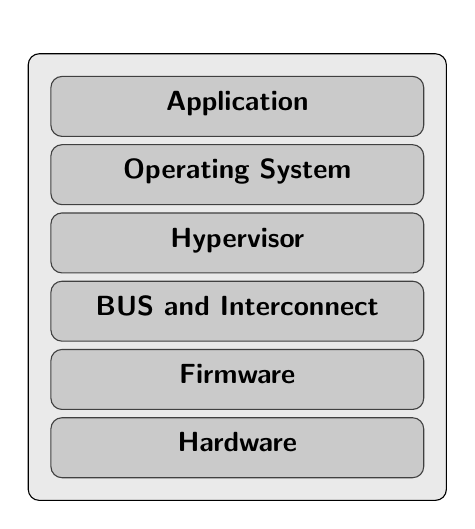
\begin{tikzpicture}[scale=0.50,node distance=3pt,outer sep=0pt,
platformlayer/.style={
  draw=darkgray,
  fill=nodecolor,
  rounded corners,
  text width=4.5cm,
  font={\sffamily\bfseries\color{black}},
  align=center,
  text height=9pt,
  text depth=6pt},
]
\node[platformlayer] (APP) {Application};
\node[platformlayer,below=of APP](OS) {Operating System};
\node[platformlayer,below=of OS] (HYP) {Hypervisor};
\node[platformlayer,below=of HYP](BUS){BUS and Interconnect};
\node[platformlayer,below=of BUS](FW) {Firmware};
\node[platformlayer,below=of FW](HW) {Hardware};

\begin{pgfonlayer}{background}
\draw[platformlayer,draw=black,fill=nodecolor!40]([xshift=-\framesep,yshift=1\framesep]current bounding box.north west)
rectangle ([xshift=\framesep,yshift=-\framesep]current bounding box.south east) 
node[below] at (0,2) {};

\end{pgfonlayer}
\end{tikzpicture}
\caption{Computing Platform Layers}
\label{fig:layers}
\end{figure}

\section{Background}
Here, we consider the diverse array of computing platforms as a number
of abstracted layers: hardware, firmware, bus, hypervisor, operating
system, application, and network layers. In this way, we can
categorize the research efforts that target each layer.

The layers are arranged from lowest to highest layer. The lower layer
has more control over the computing system, while the upper layers
have less control. For instance, the Hardware layer has total control
over the physical hardware and memory of the machine, while an
application running in the Application layer can only see a portion of
the machine's memory (because of the virtual memory used by the
Operating System).

A typical compromise, in relation to the proposed layers, is the
following: A vulnerability in an application is targeted, thus
allowing the attacker full control of the application layer. From
here, the attacker can scan the other applications on the network and
attempt to exploit those applications, thus spreading horizontally
throughout the network. Alternatively, as the application layer is the
least privileged and least persistent of the layers, the attack can
attempt to further the compromise on the lower layers of the machine.
For instance, the attacker can exploit the hypervisor layer to
compromise the host hypervisor. From this vantage point, the attacker
can transparently extract information from all the other guest
Operating Systems. More insidiously, the attacker can even exploit the
firmware level, which allows the attacker to persist even after
a complete reinstall of the operating system.

In our abstract model, the lower levels have more control over the
computing system, yet they have a smaller attacker surface. However,
the lower levels can be attacked by exploiting the upper levels. Also, the upper
levels trust the abstractions provided by the lower levels. For
instance, the application-layer visualization of an industrial control
system trusts that the data reported by the hardware layer is
accurate. If an attacker is able to control and manipulate the
hardware to falsely report the state of the system, the entire
integrity of the system can be compromised.

The interconnected nature of the layers means that the security of the
entire layer must be a priority. However, at the same time, the
security improvement of any layer will have an amplifying effect on
the security of the whole system. For instance, improvement to the
security of the application layer decreases the chance of an
application compromise, which further decreases the risk of the attack
propagating throughout the network and through the other layers.

% Head 1
\section{MMSN Protocol}

% Head 2
\subsection{Frequency Assignment}

We propose a suboptimal distribution to be used by each node, which is
easy to compute and does not depend on the number of competing
nodes. A natural candidate is an increasing geometric sequence, in
which
% Numbered Equation
\begin{equation}
\label{eqn:01}
P(t)=\frac{b^{\frac{t+1}{T+1}}-b^{\frac{t}{T+1}}}{b-1},
\end{equation}
where $t=0,{\ldots}\,,T$, and $b$ is a number greater than $1$.

In our algorithm, we use the suboptimal approach for simplicity and
generality. We need to make the distribution of the selected back-off
time slice at each node conform to what is shown in Equation
(\ref{eqn:01}). It is implemented as follows: First, a random
variable $\alpha$ with a uniform distribution within the interval
$(0, 1)$ is generated on each node, then time slice $i$ is selected
according to the following equation:
% Unnumbered Equation
\[
i=\lfloor(T+1)\log_b[\alpha(b-1)+1]\rfloor.
\]
It can be easily proven that the distribution of $i$ conforms to Equation
(\ref{eqn:01}).

So protocols [Bahl 2002,Culler 2001,Zhou 2006,Adya 2001,Culler 2001;
Tzamaloukas-01; Akyildiz-01] that use RTS/CTS
controls\footnote{RTS/CTS controls are required to be implemented by
802.11-compliant devices. They can be used as an optional mechanism
to avoid Hidden Terminal Problems in the 802.11 standard and
protocols based on those similar to [Akyildiz 2001] and
[Adya 2001].} for frequency negotiation and reservation are not
suitable for WSN applications, even though they exhibit good
performance in general wireless ad hoc
networks.

% Head 3
\subsubsection{Exclusive Frequency Assignment}

In exclusive frequency assignment, nodes first exchange their IDs
among two communication hops so that each node knows its two-hop
neighbors' IDs. In the second broadcast, each node beacons all
neighbors' IDs it has collected during the first broadcast period.

% Head 4
\paragraph{Eavesdropping}

Even though the even selection scheme leads to even sharing of
available frequencies among any two-hop neighborhood, it involves a
number of two-hop broadcasts. To reduce the communication cost, we
propose a lightweight eavesdropping scheme.

\subsection{Basic Notations}

As Algorithm~\ref{alg:one} states, for each frequency
number, each node calculates a random number (${\textit{Rnd}}_{\alpha}$) for
itself and a random number (${\textit{Rnd}}_{\beta}$) for each of its two-hop
neighbors with the same pseudorandom number generator.
% Algorithm
\begin{algorithm}[t]
\SetAlgoNoLine
\KwIn{Node $\alpha$'s ID ($ID_{\alpha}$), and node $\alpha$'s
neighbors' IDs within two communication hops.}
\KwOut{The frequency number ($FreNum_{\alpha}$) node $\alpha$ gets assigned.}
$index$ = 0; $FreNum_{\alpha}$ = -1\;
\Repeat{$FreNum_{\alpha} > -1$}{
        $Rnd_{\alpha}$ = Random($ID_{\alpha}$, $index$)\;
        $Found$ = $TRUE$\;
        \For{each node $\beta$ in $\alpha$'s two communication hops
    }{
      $Rnd_{\beta}$ = Random($ID_{\beta}$, $index$)\;
      \If{($Rnd_{\alpha} < Rnd_{\beta}$) \text{or} ($Rnd_{\alpha}$ ==
          $Rnd_{\beta}$ \text{and} $ID_{\alpha} < ID_{\beta}$)\;
      }{
        $Found$ = $FALSE$; break\;
      }
        }
     \eIf{$Found$}{
           $FreNum_{\alpha}$ = $index$\;
         }{
           $index$ ++\;
     }
      }
\caption{Frequency Number Computation}
\label{alg:one}
\end{algorithm}

Bus masters are divided into two disjoint sets, $\mathcal{M}_{RT}$
and $\mathcal{M}_{NRT}$.
% description
\begin{description}
\item[RT Masters]
$\mathcal{M}_{RT}=\{ \vec{m}_{1},\dots,\vec{m}_{n}\}$ denotes the
$n$ RT masters issuing real-time constrained requests. To model the
current request issued by an $\vec{m}_{i}$ in $\mathcal{M}_{RT}$,
three parameters---the recurrence time $(r_i)$, the service cycle
$(c_i)$, and the relative deadline $(d_i)$---are used, with their
relationships.
\item[NRT Masters]
$\mathcal{M}_{NRT}=\{ \vec{m}_{n+1},\dots,\vec{m}_{n+m}\}$ is a set
of $m$ masters issuing nonreal-time constrained requests. In our
model, each $\vec{m}_{j}$ in $\mathcal{M}_{NRT}$ needs only one
parameter, the service cycle, to model the current request it
issues.
\end{description}

Here, a question may arise, since each node has a global ID. Why
don't we just map nodes' IDs within two hops into a group of
frequency numbers and assign those numbers to all nodes within two
hops?

\section{Simulator}
\label{sec:sim}

If the model checker requests successors of a state which are not
created yet, the state space uses the simulator to create the
successors on-the-fly. To create successor states the simulator
conducts the following steps.
% enumerate
\begin{enumerate}
\item Load state into microcontroller model.
\item Determine assignments needed for resolving nondeterminism.
\item For each assignment.
      \begin{enumerate}
      \item either call interrupt handler or simulate effect of next instruction, or
      \item evaluate truth values of atomic propositions.
      \end{enumerate}
\item Return resulting states.
\end{enumerate}
Figure~\ref{fig:one} shows a typical microcontroller C program that
controls an automotive power window lift. The program is one of the
programs used in the case study described in Section~\ref{sec:sim}.
At first sight, the programs looks like an ANSI~C program. It
contains function calls, assignments, if clauses, and while loops.
% Figure
\begin{figure}
\caption{Code before preprocessing.}
\label{fig:one}
\end{figure}

\subsection{Problem Formulation}

The objective of variable coalescence-based offset assignment is to find
both the coalescence scheme and the MWPC on the coalesced graph. We start
with a few definitions and lemmas for variable coalescence.

% Enunciations
\begin{definition}[Coalesced Node (C-Node)]A C-node is a set of
live ranges (webs) in the AG or IG that are coalesced. Nodes within the same
C-node cannot interfere with each other on the IG. Before any coalescing is
done, each live range is a C-node by itself.
\end{definition}

\begin{definition}[C-AG (Coalesced Access Graph)]The C-AG is the access
graph after node coalescence, which is composed of all C-nodes and C-edges.
\end{definition}

\begin{lemma}
The C-MWPC problem is NP-complete.
\end{lemma}
\begin{proof} C-MWPC can be easily reduced to the MWPC problem assuming a
coalescence graph without any edge or a fully connected interference graph.
Therefore, each C-node is an uncoalesced live range after value separation
and C-PC is equivalent to PC. A fully connected interference graph is made
possible when all live ranges interfere with each other. Thus, the C-MWPC
problem is NP-complete.
\end{proof}

\begin{lemma}[Lemma Subhead]The solution to the C-MWPC problem is no
worse than the solution to the MWPC.
\end{lemma}
\begin{proof}
Simply, any solution to the MWPC is also a solution to the
C-MWPC. But some solutions to C-MWPC may not apply to the MWPC (if any
coalescing were made).
\end{proof}

\section{Performance Evaluation}

During all the experiments, the Geographic Forwarding (GF)
[Akyildiz 2001] routing protocol is used. GF exploits geographic
information of nodes and conducts local data-forwarding to achieve
end-to-end routing. Our simulation is
configured according to the settings in
Table~\ref{tab:one}. Each run lasts for 2 minutes and
repeated 100 times. For each data value we present in the results,
we also give its 90\% confidence interval.
% Table
\begin{table}%
\tbl{Simulation Configuration\label{tab:one}}{%
\begin{tabular}{|l|l|}
\hline
TERRAIN{$^a$}   & (200m$\times$200m) Square\\\hline
Node Number     & 289\\\hline
Node Placement  & Uniform\\\hline
Application     & Many-to-Many/Gossip CBR Streams\\\hline
Payload Size    & 32 bytes\\\hline
Routing Layer   & GF\\\hline
MAC Layer       & CSMA/MMSN\\\hline
Radio Layer     & RADIO-ACCNOISE\\\hline
Radio Bandwidth & 250Kbps\\\hline
Radio Range     & 20m--45m\\\hline
\end{tabular}}
\begin{tabnote}%
\Note{Source:}{This is a table
sourcenote. This is a table sourcenote. This is a table
sourcenote.}
\vskip2pt
\Note{Note:}{This is a table footnote.}
\tabnoteentry{$^a$}{This is a table footnote. This is a
table footnote. This is a table footnote.}
\end{tabnote}%
\end{table}%

\section{Conclusions}

In this article, we develop the first multifrequency MAC protocol for
WSN applications in which each device adopts a
single radio transceiver. The different MAC design requirements for
WSNs and general wireless ad-hoc networks are
compared, and a complete WSN multifrequency MAC design (MMSN) is
put forth. During the MMSN design, we analyze and evaluate different
choices for frequency assignments and also discuss the nonuniform
back-off algorithms for the slotted media access design.

% Start of "Sample References" section

\section{Typical references in new ACM Reference Format}
A paginated journal article \cite{Abril07}, an enumerated
journal article \cite{Cohen07}, a reference to an entire issue \cite{JCohen96},
a monograph (whole book) \cite{Kosiur01}, a monograph/whole book in a series (see 2a in spec. document)
\cite{Harel79}, a divisible-book such as an anthology or compilation \cite{Editor00}
followed by the same example, however we only output the series if the volume number is given
\cite{Editor00a} (so Editor00a's series should NOT be present since it has no vol. no.),
a chapter in a divisible book \cite{Spector90}, a chapter in a divisible book
in a series \cite{Douglass98}, a multi-volume work as book \cite{Knuth97},
an article in a proceedings (of a conference, symposium, workshop for example)
(paginated proceedings article) \cite{Andler79}, a proceedings article
with all possible elements \cite{Smith10}, an example of an enumerated
proceedings article \cite{VanGundy07},
an informally published work \cite{Harel78}, a doctoral dissertation \cite{Clarkson85},
a master's thesis: \cite{anisi03}, an online document / world wide web resource \cite{Thornburg01}, \cite{Ablamowicz07},
\cite{Poker06}, a video game (Case 1) \cite{Obama08} and (Case 2) \cite{Novak03}
and \cite{Lee05} and (Case 3) a patent \cite{JoeScientist001},
work accepted for publication \cite{rous08}, 'YYYYb'-test for prolific author
\cite{SaeediMEJ10} and \cite{SaeediJETC10}. Other cites might contain
'duplicate' DOI and URLs (some SIAM articles) \cite{Kirschmer:2010:AEI:1958016.1958018}.
Boris / Barbara Beeton: multi-volume works as books
\cite{MR781536} and \cite{MR781537}.

% Appendix
\appendix
\section*{APPENDIX}
\setcounter{section}{1}
In this appendix, we measure
the channel switching time of Micaz [CROSSBOW] sensor devices.
In our experiments, one mote alternatingly switches between Channels
11 and 12. Every time after the node switches to a channel, it sends
out a packet immediately and then changes to a new channel as soon
as the transmission is finished. We measure the
number of packets the test mote can send in 10 seconds, denoted as
$N_{1}$. In contrast, we also measure the same value of the test
mote without switching channels, denoted as $N_{2}$. We calculate
the channel-switching time $s$ as
\begin{eqnarray}%
s=\frac{10}{N_{1}}-\frac{10}{N_{2}}. \nonumber
\end{eqnarray}%
By repeating the experiments 100 times, we get the average
channel-switching time of Micaz motes: 24.3$\mu$s.

\appendixhead{ZHOU}

% Acknowledgments
\begin{acks}
The authors would like to thank Dr. Maura Turolla of Telecom
Italia for providing specifications about the application scenario.
\end{acks}

% Bibliography
\bibliographystyle{ACM-Reference-Format-Journals}
\bibliography{acmsmall-sample-bibfile}
\bibliography{papers}
                             % Sample .bib file with references that match those in
                             % the 'Specifications Document (V1.5)' as well containing
                             % 'legacy' bibs and bibs with 'alternate codings'.
                             % Gerry Murray - March 2012

% History dates
\received{February 2007}{March 2009}{June 2009}

\end{document}
% End of v2-acmsmall-sample.tex (March 2012) - Gerry Murray, ACM


